\documentclass[12pt]{article}
\usepackage[utf8]{inputenc} % uft8 you know
\usepackage[danish]{babel}
\usepackage{lastpage}
\usepackage{fancyhdr}
\usepackage{hyperref}
\usepackage{comment}
\usepackage[
backend=biber,
style=apa,
sorting=ynt
]{biblatex}
\addbibresource{sources/library.bib}
\usepackage[T1]{fontenc}
\usepackage{ae}
\usepackage{graphicx}
\usepackage{array}
\usepackage{ragged2e} % for \RaggedRight command
\usepackage{booktabs} % for \toprule, \midrule, \bottomrule
\usepackage{pdfpages} % Til at inkludere pdf'er
\usepackage{amsmath}
\usepackage{amsfonts}
\usepackage{amssymb}
\usepackage{longtable}
\usepackage{adjustbox}
\usepackage{blindtext}
\usepackage{geometry}
\usepackage{multirow}
%\usepackage{natbib} % Works with.bib files
%\bibliographystyle{apalike} 
\usepackage{tabularx, booktabs, siunitx} % From now on ist only code styling!
% Default fixed font does not support bold face
\DeclareFixedFont{\ttb}{T1}{txtt}{bx}{n}{12} % for bold
\DeclareFixedFont{\ttm}{T1}{txtt}{m}{n}{12}  % for normal
% Custom colors
\usepackage{color}
\definecolor{deepblue}{rgb}{0,0,0.5}
\definecolor{deepred}{rgb}{0.6,0,0}
\definecolor{deepgreen}{rgb}{0,0.5,0}
\newcommand\pythonstyle{\lstset{
language=Python,
basicstyle=\ttm,
morekeywords={self},              % Add keywords here
keywordstyle=\ttb\color{deepblue},
emph={MyClass,__init__},          % Custom highlighting
emphstyle=\ttb\color{deepred},    % Custom highlighting style
stringstyle=\color{deepgreen},
frame=tb,                         % Any extra options here
showstringspaces=false,
breaklines=true
}}

\usepackage{hyperref}
\usepackage{caption}
\DeclareCaptionFont{white}{\color{white}}
\DeclareCaptionFormat{listing}{\colorbox{blue}{\parbox{\textwidth}{\hspace{15pt}#1#2#3}}}
\captionsetup[lstlisting]{format=listing,labelfont=white,textfont=white, singlelinecheck=false, margin=0pt, font={bf,footnotesize}}
\usepackage{listings}

\geometry{
    a4paper,
    total={170mm,257mm},
    left=20mm,
    top=30mm,
    bottom=30mm,
}
\hypersetup{
    linkcolor=black,
    colorlinks=false,
    pdftitle={SOP - Kristoffer Frøkjær Sørensen},
    pdfauthor={Kristoffer Frøkjær Sørensen},
    % Remove the red border around links
    pdfborder={0 0 0},
}

\pagestyle{fancy} % definds the pagestyleing
\fancyhf{} % Removes the wired header text
\renewcommand{\headrulewidth}{0pt} % Removes the line under the header
\cfoot{Side \thepage\ af \pageref{LastPage}} % Sets the right side of the footer to "Page X of Y"
\lhead{Kristoffer Sørensen} % Sets the left side of the header to "Gruppe 1"

\begin{document}
    % Python environment
    \lstnewenvironment{python}[1][]
    {
    \pythonstyle
    \lstset{#1}
    }
    {}
    % Python for external files
    \newcommand\pythonexternal[2][]{{
    \pythonstyle
    \lstinputlisting[#1]{#2}}}
    % Python for inline
    \newcommand\pythoninline[1]{{\pythonstyle\lstinline!#1!}}

    \lstnewenvironment{JavaScript}[3][]
    {
    \JavaScriptStyle
    \lstset{#2}
    }
    {}

    \lstloadlanguages{C,C++,csh,Java}

\definecolor{red}{rgb}{0.6,0,0} 
\definecolor{blue}{rgb}{0,0,0.6}
\definecolor{green}{rgb}{0,0.8,0}
\definecolor{cyan}{rgb}{0.0,0.6,0.6}

\lstset{
language=csh,
basicstyle=\footnotesize\ttfamily,
numbers=left,
numberstyle=\tiny,
numbersep=5pt,
tabsize=2,
extendedchars=true,
breaklines=true,
frame=b,
stringstyle=\color{blue}\ttfamily,
showspaces=false,
showtabs=false,
xleftmargin=17pt,
framexleftmargin=17pt,
framexrightmargin=5pt,
framexbottommargin=4pt,
commentstyle=\color{green},
morecomment=[l]{//}, %use comment-line-style!
morecomment=[s]{/*}{*/}, %for multiline comments
showstringspaces=false,
morekeywords={ abstract, event, new, struct,
as, explicit, null, switch,
base, extern, object, this,
bool, false, operator, throw,
break, finally, out, true,
byte, fixed, override, try,
case, float, params, typeof,
catch, for, private, uint,
char, foreach, protected, ulong,
checked, goto, public, unchecked,
class, if, readonly, unsafe,
const, implicit, ref, ushort,
continue, in, return, using,
decimal, int, sbyte, virtual,
default, interface, sealed, volatile,
delegate, internal, short, void,
do, is, sizeof, while,
double, lock, stackalloc,
else, long, static,
enum, namespace, string},
keywordstyle=\color{cyan},
identifierstyle=\color{red}
}

    %\providecommand\NAT
    \title{
    SOP - Mindste kvadraters metode \\ 
    \large{Rybners HTX - Vejleder: Carsten Finn Sørensen og Vicki Jacob} \\
    \small{Programering B og Matematik A}
}
\author{Af Kristoffer Sørensen}
\thispagestyle{empty}
\maketitle
%\begin{figure}[h!]
  %  \centering
  %  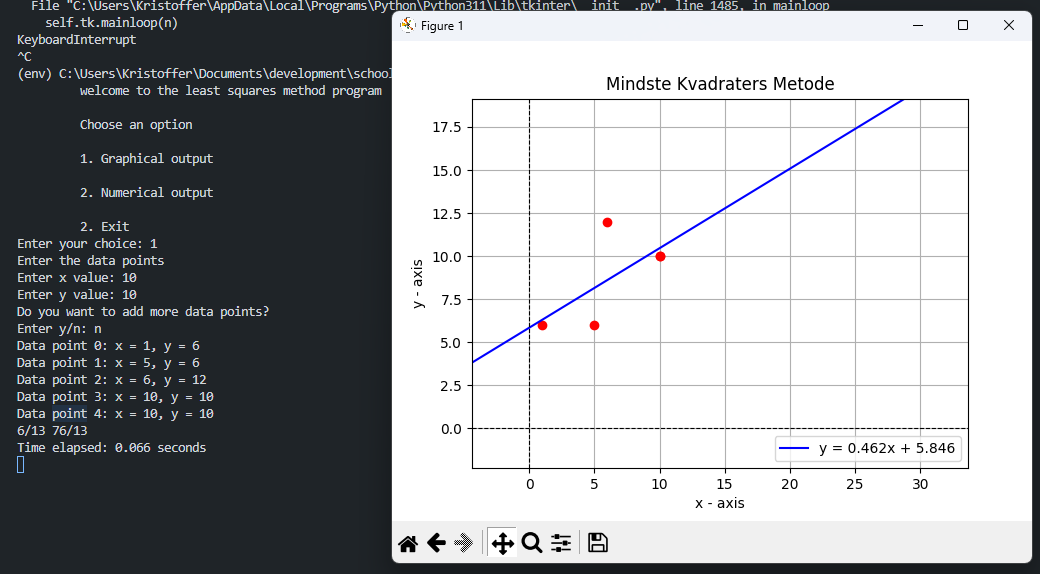
\includegraphics[width=0.9\textwidth]{figurs/forsideimg.jpg}
  %  \caption{Nuclear Bomb Explosion - Mushroom Cloud stock photo (\cite{RomoloTavani2018}) }%\cite{Forsideimg}} TODO: Add source
 %   \label{fig:Forsideimg}
%\end{figure}
\newpage
    \section*{Resume}
Denne opgave undersøger anvendelsen af Mindste Kvadraters Metode til at modellere data og ved hjælp af det, finde den bedst passende funktion. Metoden er baseret på matematikken bag funktioner af to variable og partiel differentiation. Partiel differentiation bruges her til at finde et minimumspunkt hvilket gør det muligt at finde det sted hvor summen af kvadraternes areal mellem datapunkter og en lineær linje er mindst. Den teoretiske forståelse blev omsat til praksis ved anvendelse på et datasæt og implementering i Python. I programmeringskonteksten blev metoden implementeret med fokus på modularitet og brugervenlighed, en pseudokode blev lavet for at strukturere processen. Fordelene ved programmering inkluderer hurtigere beregninger, automatisering og muligheden for at håndtere store datasæt, men udfordringer som fejl i input og beregnings hastighed ved store datasæt bliver også belyst. En diskussionen om kodningsmetoder fremhævede forskellene mellem procedural, objektorienterede og funktionel programmerings tilgange, hvor valget af metode afhænger af projektets kompleksitet og skalerbarhed. Der blev desuden også diskuteret hvilke kontrolstrukture der er bedst i hvilke senarier. Samlet set demonstrerer opgaven, hvordan Mindste Kvadraters Metode i kombination med programmering kan omsætte komplekse matematiske beregninger til effektive og anvendelige løsninger i dataanalyse. \newpage
    \tableofcontents

\newpage
    \section{Indledning}\label{sec:indledning}
I en verden, hvori data spiller en central rolle, er evnen til at analysere og modellere datasæt afgørende for videnskabelig forskning, og genrelt tolkning af datasæt. For at kunne analysere data er det nødvendigt at kunne finde en model, der beskriver sammenhængen mellem de forskellige variable. En af de metoder der kan anvendes til at beskrive data er Mindste Kvardraters Metode. Denne metode gør det muligt, at finde den best mulige funktion, ved at funktionstilpassse. Mindste Kvardraters Metode er især nyttig når man arbejder med lineære regression hvor målet er at finde en ret linje. Der bedst beskriver sammenhængen mellem to variable. Ved at anvende denne metode kan man nemt finde og forudsige tendenser i værdier baseret på allerede eksisernede data. For at forstå anvendelsen af Mindste Kvardraters Metode er det nødvendigt at dykke ned i de del elementer der ingår. Herunder funktioner af to variable og det at partiellt aflede noget. Dette giver en god teoretisk baggrund for at implementere metoden effektivt i en programerings kontekst. % Måske tilføje dette: Denne opgave vil undersøge, hvordan Mindste Kvadraters Metode kan bruges til at modellere datasæt og forudsige tendenser. Gennem en teoretisk redegørelse og praktisk implementering vil der blive vist, hvordan metoden fungerer, og hvilke fordele og begrænsninger der følger med dens anvendelse.
\section{Opgaveformulering}\label{sec:opgaveformulering}
Hvordan kan Mindste Kvadraters Metode anvendes til at modellere data for at finde den bedst mulige funktionstilpasning?
\begin{itemize}
    \item Redegør for matematikken bag mindste kvadraters metode, herunder skal der redegøres for funktioner med to variabler og de partielle afledede.
    \item Anvend mindste kvadraters metode på et selvvalgt datasæt.
    \item Producer et eksempel på implementering af mindste kvadraters metode.
    \item Vurder hvilke fordele og begrænsninger der følger med denne metode i en programmeringskontekst.
    \item Diskuter forskellige kodningsmetoder til løsning af mindste kvadraters metode. 
\end{itemize}
\newpage
    \section{Regresionsanalyse?}\label{sec:regresionsanalyse}
Regressionsanalyse er en statistisk metode, der anvendes til at undersøge og modellere sammenhæng mllem en afhængig variabel og en uafhængig variabel. Denne metode er udbredt inden for områder som økonomi, sunhed- og samfunds forskning samt naturvidenskaben. Historisk set blev beregningerne udført manuelt, hvilket var både tidskrævende og tilbøjeligt til at give fejl. Den frøste version af regresionsanalyse blev for første gang nævnt i en artikel af Francis Galton i år 1886. Francis Galton var en engelsk videnskabsmand. Francis Galton var blandt andet kendt for at være opfinderen af fingeraftryks identificering. Den metode som Francis Galton beskrev, er i dag kendt som Regression mod gennemsnittet. Begræbet beskriver at hvis en variabel er langt fra gennemsnittet, så vil den næste værdi af samme variabel være tættere på gennemsnittet. Galton målte højden på 250 forældre og deres 930 voksene børn. Han justerede møderenes højde ved at gange med 1,08 Forældernes højde var morens og farens højde delt med to. Hr. Galton sikere sig at der ikke vare en systemmatisk tendenst til at høje mænd giftede sig med høje kvinder og at lave mænd gitede sig med lave kvinder. Plotte han sine obeservationer ind i et kordinatsystem hvor han hen af x-aksen havde Forældernes højde og ad y-aksen havde han børnenes højde. Galton troede, han havde gjort sig en stor opdagelse. Han fandt ud af at sønner af meget høje fædre ofte var højere end gemmensnittet, men dog stadig lavere end deres fædre. Det så ud som om at der var en ukendt faktor, der var skyld i at menneskets højde bevlgede sig væk fra det ekstremt høje ned til det mere normale gennemsnit. Det fænomen kaldte han ”regression towards mediocrity” (”tilbagevenden til middel-mådelighed”) % KILDE: https://lex.dk/regression_mod_gennemsnittet og https://lru.praxis.dk/Lru/microsites/hvadermatematik/hem3download/kap8_QR5b_Galton_Regression_towards_the_mean.pdf
Selvom at Galtons opdagelse var banebryende og introducerede begræbet regression, anvendes denne metode ikke længere. Hans tilgang var basseret på specefikke observationer, så som netop højde, dette betød at man manglede den matematiske tilgang. Galtons bidrag dannede dog fundament for videreudviklingen af regressionsmetoder. I dag bygger regressionsanalyse på et stærkt matematisk og statistisk fundament. Dette fundament blev blandt andet bygget af Carl Fredrich Gauss og Adrien.Marie Legendre, der introducerede mindste kvardraters metode. Denne metode, spiller stadig en central rolle i regressionsanalyser. Der er mange fordele ved at anvende regresionsanalyse, men der er dog også en del ulemper ved det. Metoden forudsætter at dine data kan beskrives som en funktion, at dine data reelt 
% Hvad er Mindste Kvadraters Metode? Hvad kan den anvendes til? (Også praktisk!) Hvad er dens begrænsninger? (Historisk, hvad med gamle dage)
\subsection{Matematikken bag Mindste Kvadraters Metode}
% Redegør for matematikken bag Mindste Kvadraters Metode

\subsubsection{Funktioner med to variabler}
Du har måske stiftet bekendskab med funktioner af en variabel. Disse funktioner er ofte skrevet som \begin{math}f(x) = x^2\end{math} eller \begin{math}g(x) = 2x + 3\end{math}. Her er ønsker man at finde værdien $f(x)$ eller $g(x)$ for et givet $x$ værdi. Her giver man altså en værdi og for en værdi tilbage. Men hvad nu, hvis du i stedet giver funktionen to tal på en gang? Hvis du for eksempel har brug for at beskrive noget  der afhænger af både $x$ og $y$? Her kommer funktioner med to variabler ind i billedet. 
% Redegør for funktioner med to variabler (Forklar forskellen mellem en- og to-dimensionelle funktioner) Introduktion til funktioner af to variable.

\subsubsection{Partielle afledede}
% Redegør for de partielle afledede

\subsection{Anvendelse af Mindste Kvadraters Metode}
% Vis hvordan Mindste Kvadraters Metode kan anvendes på et selvvalgt datasæt (Husk en fortolkning af resultaterne)


\section{Implementering af Mindste Kvadraters Metode}
% Anvend pseudokode til at vise hvordan Mindste Kvadraters Metode kan implementeres


\subsection{Program Design}
% Forklar hvilke overvejelser der er gjort i forhold til program design, sprogvalg, biblioteker, etc. Teorisk baggrund!!!

\subsection{Program redegørsel}
% Redegør for programmet og dets funktioner (Husk at inkludere kodeeksempler)

\section{Fordele og Begrænsninger}
%Her analyseres metoden på et bredere niveau ved at vurdere dens styrker og svagheder i en programmeringssammenhæng.

\section{Diskussion af Kodningsmetoder}
% While loops, for loops, rekursive funktioner, ect.

    \input{chapters/06Konklusion.tex}
    %\bibliography{sources/library}\printbibliography
    \newpage
    \printbibliography[heading=bibintoc, title={Litteratur}]
    \newpage

\section{Bilag}\label{sec:Bilag}
\subsection{Bilag 1: Koden}\label{sec:koden}
\begin{python}
    from sympy import symbols, solve, Eq, diff
import matplotlib.pyplot as plt
import numpy as np 
import time

def leastSquaresMethod(dataPoints):
    startTime = time.time() # Gets the current time
    a, b = symbols('a b')
    sumA2 = 0 # Sum of a^2 
    sumB2 = 0 # Sum of b^2
    sumAB = 0 # Sum of 2ab
    sumA = 0 # Sum of 2ax
    sumB = 0 # Sum of 2by
    sumConstant = 0
    n = len(dataPoints) # Gets the number of data points

    for i in range(n): # Loops through all data points and calculates the sums
        x = dataPoints[i][0] # Gets the x value of the data point
        y = dataPoints[i][1] # Gets the y value of the data point
        print(f"Data point {i}: x = {x}, y = {y}") # Prints what data point is being calculated
        sumA2 += a**2 * x**2 # Adds the sum of a^2
        sumB2 += b**2      # Adds the sum of b^2
        sumAB += 2*a*b*x   # Adds the sum of 2ab
        sumA += 2*a*x*y   # Adds the sum of 2ax
        sumB += 2*b*y    # Adds the sum of 2by
        sumConstant += 2*y # Adds the sum of 2c

    # Defines the function of two variabel containing the sum of squared errors
    f = sumA2 + sumB2 + sumAB - sumA - sumB + sumConstant 

    # Solve for a and b
    diffA = diff(f, a) # Differentiates f to a
    diffB = diff(f, b) # Differentiates f to b
    solutions = solve([diffA, diffB], (a, b)) # Solves the equations
    print(solutions[a], solutions[b]) # Prints the solutions
    timeElapsed = time.time() - startTime # Calculates the time elapsed
    print(f"Time elapsed: {timeElapsed:.3f} seconds") # Prints the time elapsed
    return solutions[a], solutions[b] # Returns the solutions as a tuple containing a and b [a, b]

def plotter(dataPoints):
    line = leastSquaresMethod(dataPoints) # Calls the leastSquaresMethod function and stores the result in line
    slope = float(line[0])  # Gets the slope of the line
    intercept = float(line[1])  # Gets the intercept of the line
    
    for point in dataPoints: # Loops through all data points and plots them
        plt.plot(point[0], point[1], 'ro')
    
    # Defince x values for the line
    x = np.linspace(-10, 100, 100)  # Creates a interval of the line. The line will be drawn from -10 to 100
    y = slope * x + intercept # Calculates the y values for the line
    
    # Plot linjen
    plt.plot(x, y, label=f"y = {slope:.3f}x + {intercept:.3f}", color='blue') # Plots the line
    plt.quiver(x[0], y[0], -1, -slope, angles='xy', scale_units='xy', scale=1, color='blue', width=0.003) # Adds an arrow to the start of the line
    plt.quiver(x[-1], y[-1], 1, slope, angles='xy', scale_units='xy', scale=1, color='blue', width=0.003) # Adds an arrow to the end of the line
    
    # Akse og grid
    plt.axhline(0, color='black', linewidth=0.8, linestyle='--') # Adds a horizontal line at y = 0
    plt.axvline(0, color='black', linewidth=0.8, linestyle='--') # Adds a vertical line at x = 0
    plt.title('Mindste Kvadraters Metode') # Adds a title to the plot
    plt.xlabel('x - axis') # Adds a label to the x-axis
    plt.ylabel('y - axis') # Adds a label to the y-axis
    plt.legend() # Adds a legend to the plot
    plt.grid() # Adds a grid to the plot
    plt.show() # Shows the plot

def main():
    print("\t welcome to the least squares method program")
    print("\n \t Choose an option")
    print("\n \t 1. Graphical output")
    print("\n \t 2. Numerical output")
    print("\n \t 2. Exit")
    userInput = input("Enter your choice: ")
    if userInput == "1":
        print("Enter the data points")
        dataPoints = [(1, 6), (5, 6), (6, 12), (10,10)]
        while True:
            x = input("Enter x value: ")
            y = input("Enter y value: ")
            dataPoints.append((int(x), int(y)))
            print("Do you want to add more data points?")
            choice = input("Enter y/n: ")
            if choice == "n":
                break
        plotter(dataPoints)
        main()
    elif userInput == "2":
        while True:
            x = input("Enter x value: ")
            y = input("Enter y value: ")
            dataPoints.append((int(x), int(y)))
            print("Do you want to add more data points?")
            choice = input("Enter y/n: ")
            if choice == "n":
                break
        plotter(dataPoints)
        main()
    elif userInput == "3":
        exit()
    else:
        print("Invalid input")
        main()

main()
\end{python}
\end{document}